\documentclass[11pt]{article} 
\usepackage[english]{babel}
\usepackage[utf8]{inputenc}
\usepackage[margin=0.5in]{geometry}
\usepackage{amsmath}
\usepackage{amsthm}
\usepackage{amsfonts}
\usepackage{amssymb}
\usepackage[usenames,dvipsnames]{xcolor}
\usepackage{graphicx}
\usepackage[siunitx]{circuitikz}
\usepackage{tikz}
\usepackage[colorinlistoftodos, color=orange!50]{todonotes}
\usepackage{hyperref}
\usepackage[numbers, square]{natbib}
\usepackage{fancybox}
\usepackage{epsfig}
\usepackage{soul}
\usepackage[framemethod=tikz]{mdframed}
\usepackage[shortlabels]{enumitem}
\usepackage[version=4]{mhchem}
\usepackage{multicol}
 
\usepackage{mathtools}
\usepackage{comment}
\usepackage{enumitem}
\usepackage[utf8]{inputenc}
\usepackage[linesnumbered,ruled,vlined]{algorithm2e}
\usepackage{listings}
\usepackage{color}
\usepackage[numbers]{natbib}
\usepackage{subfiles}
\usepackage{tkz-berge}


\newtheorem{prop}{Proposition}[section]
\newtheorem{thm}{Theorem}[section]
\newtheorem{lemma}{Lemma}[section]
\newtheorem{cor}{Corollary}[prop]

\theoremstyle{definition}
\newtheorem{definition}{Definition}

\theoremstyle{definition}
\newtheorem{required}{Problem}

\theoremstyle{definition}
\newtheorem{ex}{Example}


\setlength{\marginparwidth}{3.4cm}
%#########################################################

%To use symbols for footnotes
\renewcommand*{\thefootnote}{\fnsymbol{footnote}}
%To change footnotes back to numbers uncomment the following line
%\renewcommand*{\thefootnote}{\arabic{footnote}}

% Enable this command to adjust line spacing for inline math equations.
% \everymath{\displaystyle}

% _______ _____ _______ _      ______ 
%|__   __|_   _|__   __| |    |  ____|
%   | |    | |    | |  | |    | |__   
%   | |    | |    | |  | |    |  __|  
%   | |   _| |_   | |  | |____| |____ 
%   |_|  |_____|  |_|  |______|______|
%%%%%%%%%%%%%%%%%%%%%%%%%%%%%%%%%%%%%%%

\title{
\normalfont \normalsize 
\textsc{CSCI 3104 Spring 2022 \\ 
Instructors: Profs. Chen and Layer} \\
[10pt] 
\rule{\linewidth}{0.5pt} \\[6pt] 
\huge Quiz 22 - DP: Backtracking to find solution \\
\rule{\linewidth}{2pt}  \\[10pt]
}
%\author{Your Name}
\date{}

\begin{document}
\definecolor {processblue}{cmyk}{0.96,0,0,0}
\definecolor{processred}{rgb}{200, 0, 0}
\definecolor{processgreen}{rgb}{0, 255, 0}
\DeclareGraphicsExtensions{.png}
\DeclareGraphicsExtensions{.gif}
\DeclareGraphicsExtensions{.jpg}

\maketitle


%%%%%%%%%%%%%%%%%%%%%%%%%
%%%%%%%%%%%%%%%%%%%%%%%%%%
%%%%%%%%%%FILL IN YOUR NAME%%%%%%%
%%%%%%%%%%AND STUDENT ID%%%%%%%%
%%%%%%%%%%%%%%%%%%%%%%%%%%
\noindent
Due Date \dotfill April 8 \\
Name \dotfill \textbf{Chengming Li} \\
Student ID \dotfill \textbf{109251991} \\


\tableofcontents

\section{Instructions}
 \begin{itemize}
	\item The solutions \textbf{should be typed}, using proper mathematical notation. We cannot accept hand-written solutions. \href{http://ece.uprm.edu/~caceros/latex/introduction.pdf}{Here's a short intro to \LaTeX.}
	\item You should submit your work through the \textbf{class Canvas page} only. Please submit one PDF file, compiled using this \LaTeX \ template.
	\item You may not need a full page for your solutions; pagebreaks are there to help Gradescope automatically find where each problem is. Even if you do not attempt every problem, please submit this document with no fewer pages than the blank template (or Gradescope has issues with it).

	\item You \textbf{may not collaborate with other students}. \textbf{Copying from any source is an Honor Code violation. Furthermore, all submissions must be in your own words and reflect your understanding of the material.} If there is any confusion about this policy, it is your responsibility to clarify before the due date. 

	\item Posting to \textbf{any} service including, but not limited to Chegg, Discord, Reddit, StackExchange, etc., for help on an assignment is a violation of the Honor Code.

\end{itemize}

\newpage
\section{Standard 22 - DP: Backtracking to find solution}

\begin{required} \label{Problem2}
Recall the sequence alignment problem where the cost of {\em sub} and the cost of {\em indel} are all $1$ (the cost of a no-op is 0). Given the following table of optimal cost of aligning the strings EXPON and POLYN, draw the backward path consisting of backward edges to find the minimal-cost set of edit operations that transforms EXPON to POLYNO. Besides indicating the backward path, you must also give the minimal-cost set of edit operations. If there are multiple solutions, you only need to give one of them. 

\[
\begin{array}{c|ccccccc}
   & - & P & O & L & Y & N \\ \hline
 - & 0 & 1 & 2 & 3 & 4 & 5   \\
E & 1 & 1 & 2 & 3 & 4 & 5  \\
X & 2 & 2 & 2 & 3 & 4 & 5  \\
P & 3 & 2 & 3 & 3 & 4 & 5  \\
O & 4 & 3 & 2 & 3 & 4 & 5  \\
N & 5 & 4 & 3 & 3 & 4 & 4 
\end{array}
\]

\end{required}

\begin{proof}[Answer]
\begin{center}
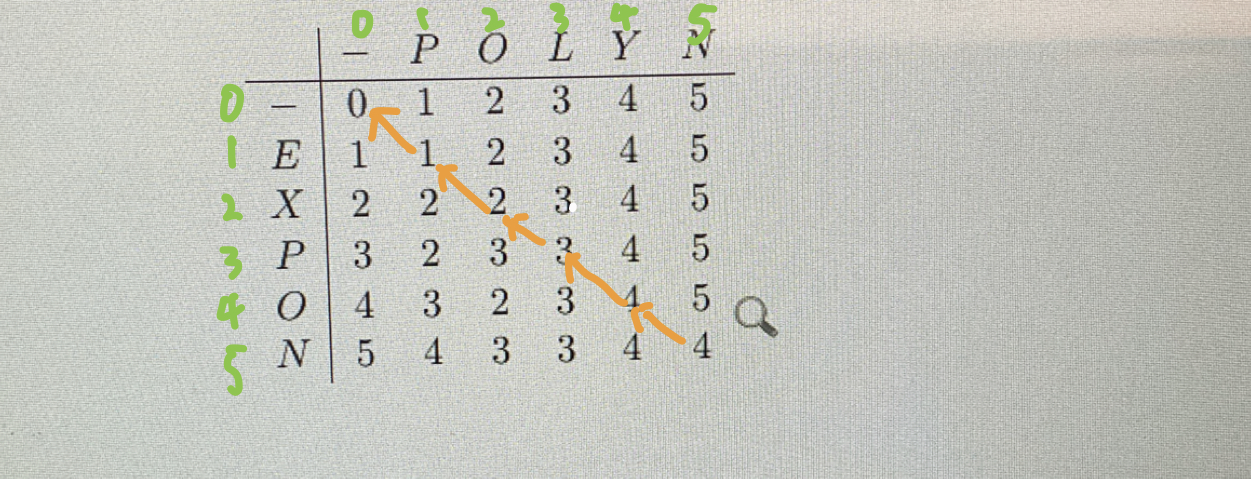
\includegraphics[width=0.7\textwidth]{IMG_0510.PNG}
\end{center}
\textbf{The path is $cost(5,5) -> cost(4,4) -> cost(3,3) -> cost(2,2) -> cost(1,1) -> cost(0,0) $}\\
\begin{align*}
cost(i,j) = min\begin{cases}
cost(i-1,j-1) + c(sub) \\
cost(i-1,j) + c(indel) \\
cost(i,j-1) + c(indel)\\
cost(i-1,j-1) & if (x_i = y_j)
\end{cases}
\end{align*}
\\\textbf{cost(5,5) = cost(4,4)+0(no-op) = 4 because it is the minimum cost and $x_i = y_j$}\\
\begin{align*}
cost(5,5) = min\begin{cases}
cost(4,4) + c(sub) = 5 \\
cost(4,5) + c(indel) = 6\\
cost(5,4) + c(indel) = 5\\
cost(4,4) = 4 & if (x_i = y_j)
\end{cases}
\end{align*}
\\\textbf{cost(4,4) = cost(3,3)+1(sub) = 4 because it is the minimum cost and $x_i \neq  y_j$}\\
\begin{align*}
cost(4,4) = min\begin{cases}
cost(3,3) + c(sub) = 4 \\
cost(3,4) + c(indel) = 5\\
cost(4,3) + c(indel) = 4\\
cost(3,3) = 3 & if (x_i = y_j)
\end{cases}
\end{align*}
\\\textbf{cost(3,3) = cost(2,2)+1(sub) = 3 because it is the minimum cost and $x_i \neq y_j$}\\
\begin{align*}
cost(3,3) = min\begin{cases}
cost(2,2) + c(sub) = 3 \\
cost(2,3) + c(indel) = 4\\
cost(3,2) + c(indel) = 4\\
cost(2,2) = 2 & if (x_i = y_j)
\end{cases}
\end{align*}
\textbf{cost(2,2) = cost(1,1)+1(sub) = 2 because it is the minimum cost and $x_i \neq  y_j$}\\
\begin{align*}
cost(2,2) = min\begin{cases}
cost(1,1) + c(sub) = 2 \\
cost(1,2) + c(indel) = 3\\
cost(2,1) + c(indel) = 3\\
cost(1,1) = 1 & if (x_i = y_j)
\end{cases}
\end{align*}
\textbf{cost(1,1) = cost(0,0)+1(sub) = 1 because it is the minimum cost and $x_i \neq  y_j$}\\
\begin{align*}
cost(1,1) = min\begin{cases}
cost(0,0) + c(sub) = 1 \\
cost(0,1) + c(indel) = 2\\
cost(1,0) + c(indel) = 2\\
cost(0,0) = 0 & if (x_i = y_j)
\end{cases}
\end{align*}
\end{proof}
%%%%%%%%%%%%%%%%%%%%%%%%%%%%%%%%%%%%%%%%%%%%%%%%%%
\end{document} % NOTHING AFTER THIS LINE IS PART OF THE DOCUMENT



